% --------------------------------------------------------------------------
% Template for DCASE 2017 paper; to be used with:
%          dcase2017.sty  - DCASE 2017 LaTeX style file, and
%          IEEEbib.bst - IEEE bibliography style file.
% Adapted from spconf.sty and waspaa15.sty
% --------------------------------------------------------------------------

\documentclass{article}
\usepackage{dcase2017,amsmath,graphicx,url,times,booktabs, tabularx}

% Example definitions.
% --------------------
\def\defeqn{\stackrel{\triangle}{=}}
\newcommand{\symvec}[1]{{\mbox{\boldmath $#1$}}}
\newcommand{\symmat}[1]{{\mbox{\boldmath $#1$}}}

% Title.
% --------------------
\title{AUTHOR GUIDELINES FOR DCASE2017 WORKSHOP MANUSCRIPTS}

% Single addresses (uncomment and modify for single-address case).
% --------------------
% \name{Author(s) Name(s)\thanks{Thanks to XYZ agency for funding.}}
% \address{Author Affiliation(s)}
%
% For example:
% ------------
% \address{School\\
%       Department\\
%       Address}

% Two addresses
% --------------------
%\twoauthors
%  {John Doe\sthanks{Thanks to ABC agency for funding.}}
%    {Fictional University\\
%Computer Science Dept., 2133 Long Road\\
%     Gotham, NY 10027, USA \\
%     john@fictional.edu}
%  {Maria Ortega\sthanks{Thanks to XYZ agency for funding.}}
%    {  University of the Imagination \\
%     Big Engineering Building, 8765 Dream Blvd. \\
%     New Chicago, IL 60626, USA \\
%     maria@imagination.edu}

% Authors in two lines, use in case of many authors with many affiliations (uncomment and modify).
% --------------------
 \name{Fabio Vesperini$^{1}$,
       Diego Droghini$^{1}$,
       Daniele Ferretti$^{1}$
       }
 \secondlinename{	
 	   Emanuele Principi$^{1}$,  
       Stefano Squartini$^{1}$, 
       Leonardo Gabrielli$^{1}$,
       Francesco Piazza$^{1}$
       }
       % fixed *.sty to allow names on multiple lines
 \address{$^1$ Politecnic University of Marche, Information Engineering  Dept., Ancona, Italy,\\ \{d.droghini, v.vesperini, d.ferretti\}@pm.univpm.it\\   
 		\{e.principi, s.squartini, l.gabrielli, f.piazza\}@univpm.it\\       
}
  

\begin{document}

\ninept
\maketitle

\begin{sloppy}

\begin{abstract}

\end{abstract}

\begin{keywords}
One, two, three, four, five
\end{keywords}


\section{Introduction}
\label{sec:intro}



\section{Sound Event Detection}
\label{sec:format}



\section{Convolutional Neural Network}
\label{sec:pagelimit}



\section{Multiscale resolution Approach}
\label{sec:pagestyle}

\subsection{First Stage}
\subsection{Second Stage}
\section{Results}
\label{sec:typestyle}

\subsection{Real Scenario application}


\section{Conclusion}
\label{sec:majhead}


Fig.~\ref{fig:results}. 

% Below is an example of how to insert images. 
% -------------------------------------------------------------------------
\begin{figure}[t]
  \centering
  \centerline{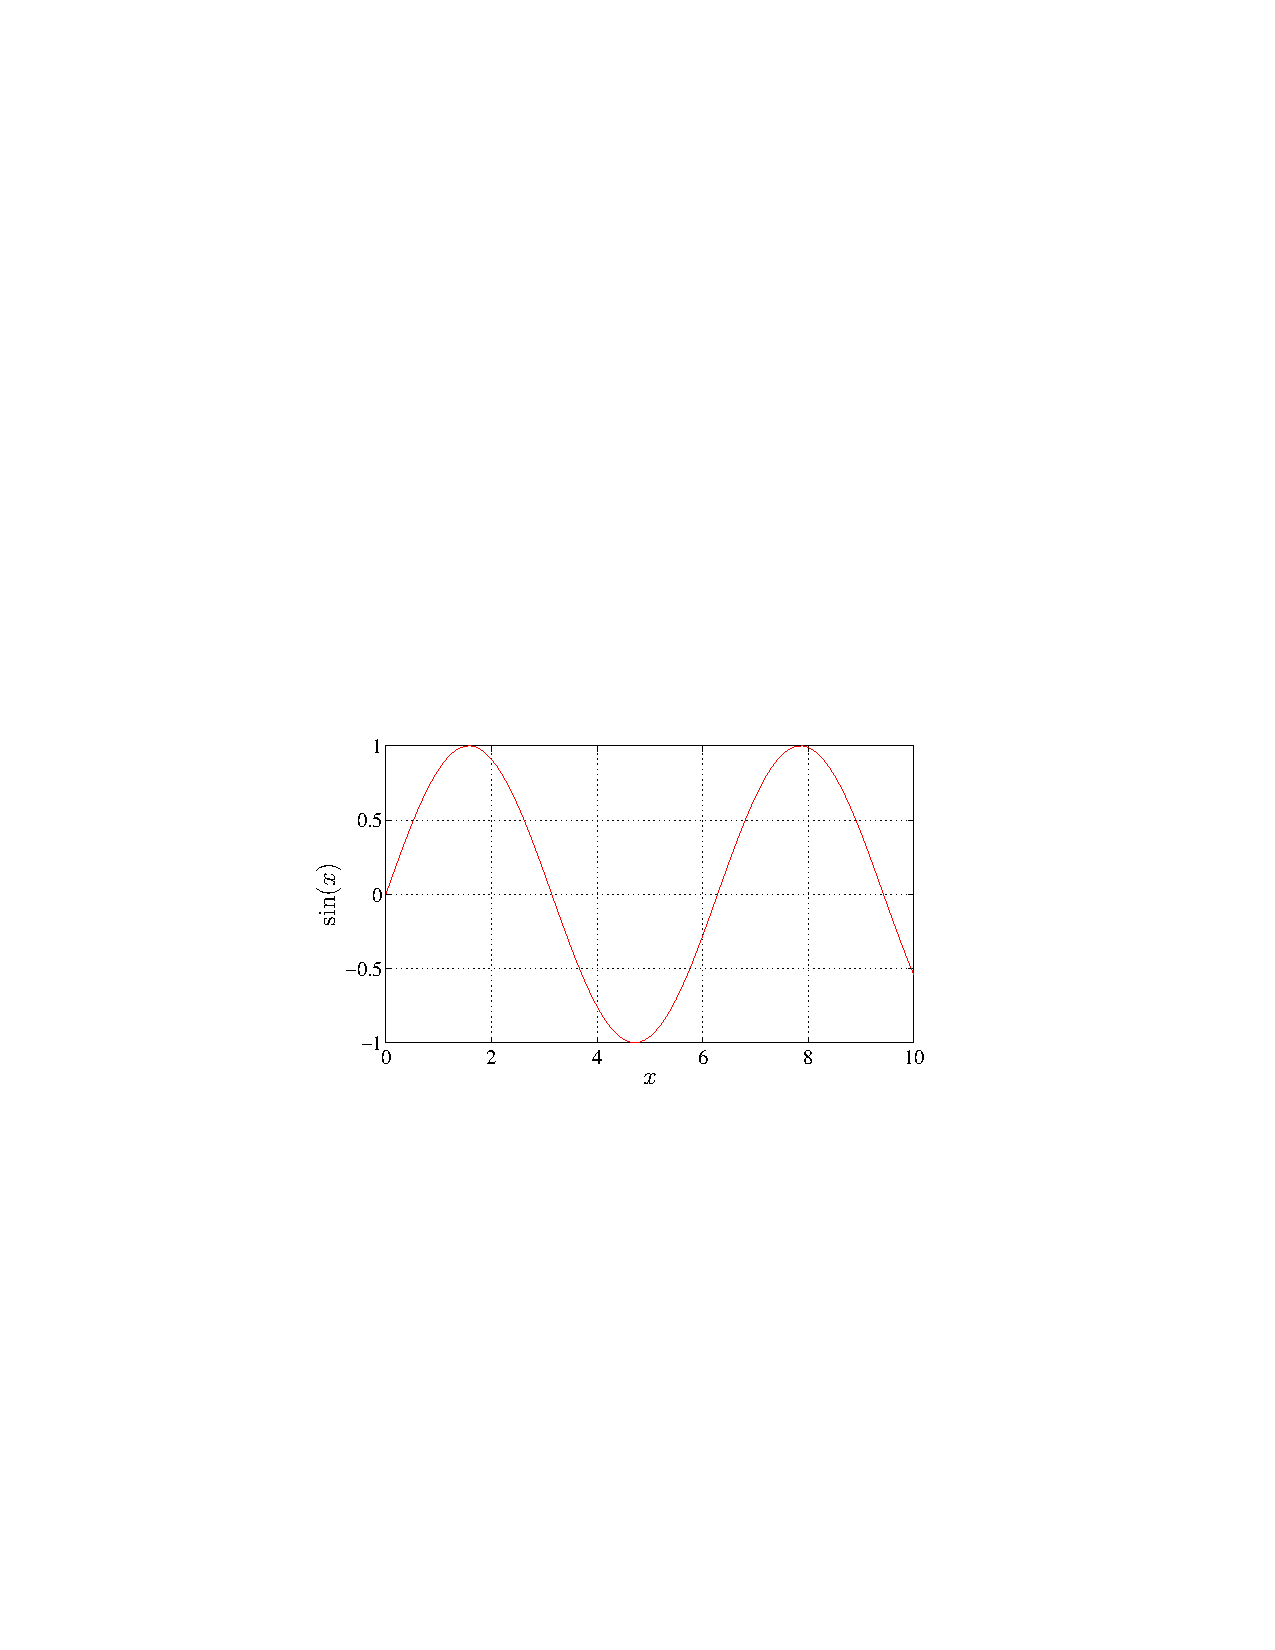
\includegraphics[width=\columnwidth]{fig1a}}
  \caption{Example of a figure with experimental results.}
  \label{fig:results}
\end{figure}

\begin{equation}
  \label{eqn:wave_equation}
    \Delta^2p(x,y,z,t)-
    \displaystyle\frac{1}{c^2}\frac{\partial^2p(x,y,z,t)}{\partial t^2}=0,
\end{equation}



% -------------------------------------------------------------------------
% Either list references using the bibliography style file IEEEtran.bst
\bibliographystyle{IEEEtran}
\bibliography{refs}
%
% or list them by yourself
% \begin{thebibliography}{9}
% 
% \bibitem{dcase2016web}
%   \url{http://www.cs.tut.fi/sgn/arg/dcase2016/}.
%
% \bibitem{IEEEPDFSpec}
%   {PDF} specification for {IEEE} {X}plore$^{\textregistered}$,
%   \url{http://www.ieee.org/portal/cms_docs/pubs/confstandards/pdfs/IEEE-PDF-SpecV401.pdf}.
%
% \bibitem{PDFOpenSourceTools}
%   Creating high resolution {PDF} files for book production with 
%   open source tools, 
%   \url{http://www.grassbook.org/neteler/highres_pdf.html}.
%
% \bibitem{eWilliams1999}
% E. Williams, \emph{Fourier Acoustics: Sound Radiation and Nearfield Acoustic
%   Holography}. London, UK: Academic Press, 1999.
% 
% \bibitem{ieeecopyright}
%   \url{http://www.ieee.org/web/publications/rights/copyrightmain.html}.
%
% \bibitem{cJones2003}
% C. Jones, A. Smith, and E. Roberts, ``A sample paper in conference
%   proceedings,'' in \emph{Proc. IEEE ICASSP}, vol. II, 2003, pp. 803--806.
% 
% \bibitem{aSmith2000}
% A. Smith, C. Jones, and E. Roberts, ``A sample paper in journals,'' 
%   \emph{IEEE Trans. Signal Process.}, vol. 62, pp. 291--294, Jan. 2000.
% 
% \end{thebibliography}


\end{sloppy}
\end{document}
\grid
